\newcommand{\tfunc}{T} %function name for the teacher
\section{\fwlfull}
\label{sec:fidelity_weighted_learning}

In this section, we address the second research question of this chapter:
\resq{c5.2}

We introduce \fwlfull (\fwl), a Bayesian semi-supervised approach that leverages a small amount of data with strong labels to generate a larger training set with \emph{confidence-weighted weakly-labeled samples}, which can then be used to modulate the fine-tuning process based on the fidelity (or quality) of each weak sample. By directly modeling the inaccuracies introduced by the \wa in this way, we can control the extent to which we make use of this additional source of weak supervision: more for confidently-labeled weak samples close to the true observed data, and less for uncertain samples further away from the observed data. We use a non-parametric kernel-based method to measure the closeness.

We propose a setting consisting of two main modules. One is called the \std and is in charge of learning a suitable data representation and performing the main prediction task (similar to the \tnet in Section~\ref{sec:meta_learning}), the other is the \tch which modulates the learning process by modeling the inaccuracies in the labels. 

\begin{figure}[!t]%
    \makebox[\textwidth][c]{
    \centering
    \begin{subfigure}[t]{0.325\textwidth}
        \centering
        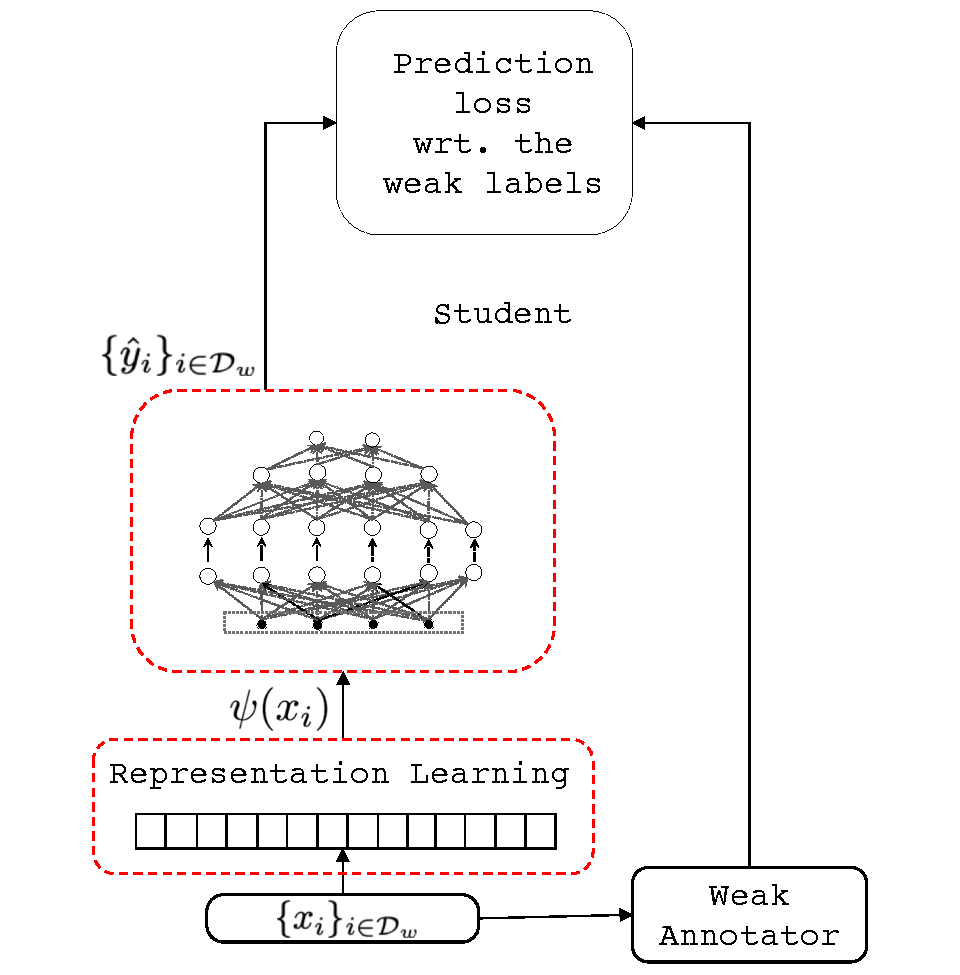
\includegraphics[width=\textwidth]{03-part-02/chapter-05/figs_and_tables/fig_fwl_step_1.pdf}
        \caption{\label{fig:step1}Step 1}
    \end{subfigure}%
    ~
    \begin{subfigure}[t]{0.25\textwidth}
        \centering
        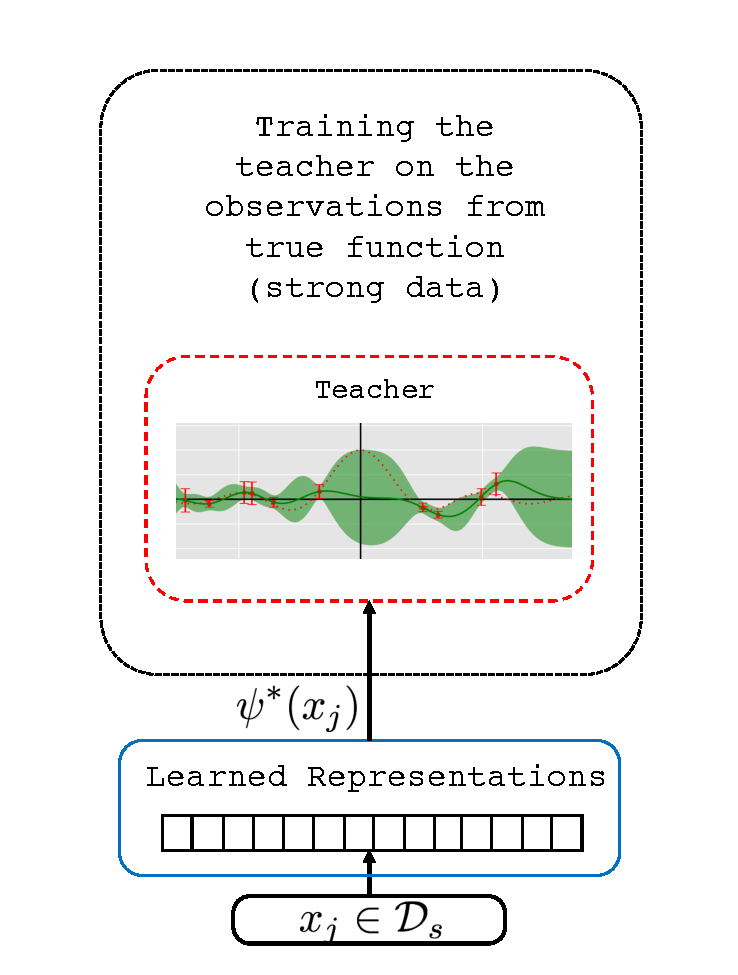
\includegraphics[width=\textwidth]{03-part-02/chapter-05/figs_and_tables/fig_fwl_step_2.pdf}
        \caption{\label{fig:step2}Step 2}
    \end{subfigure}%
     ~
    \begin{subfigure}[t]{0.425\textwidth}
        \centering
        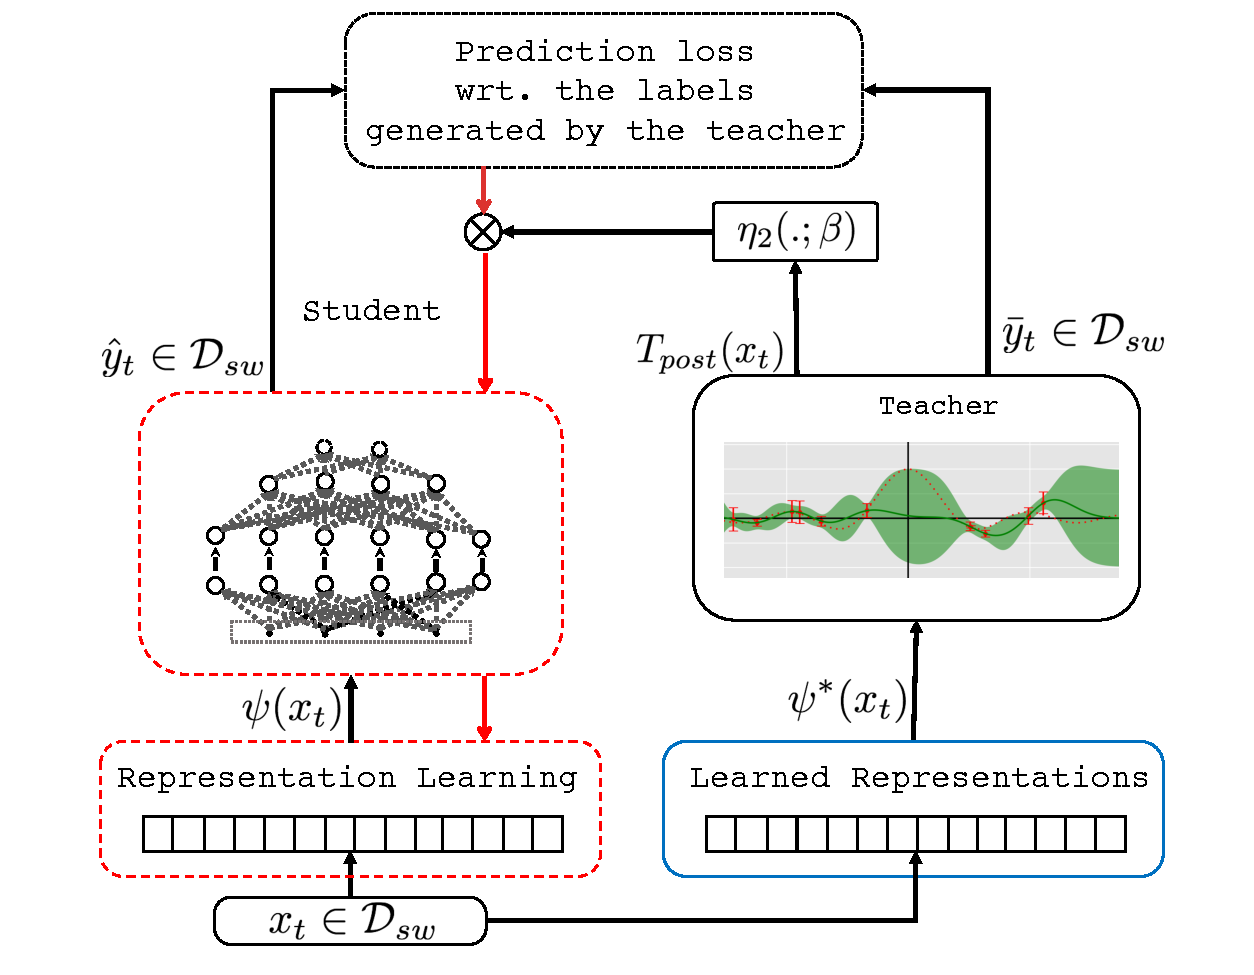
\includegraphics[width=\textwidth]{03-part-02/chapter-05/figs_and_tables/fig_fwl_step_3.pdf}
        \caption{\label{fig:step3}Step 3}
    \end{subfigure}%
    }
    \caption{Illustration of \fwlfull: Step 1: Pre-train \std on weak data,  Step 2: Fit \tch to observations from the true function, and Step 3: Fine-tune \std on labels generated by \tch, taking the confidence into account. Red dotted borders and blue solid borders depict components with trainable and non-trainable parameters, respectively.}
    \label{fig:model_fwl}
\end{figure}
\subsection{Recipe of the \fwlfull}
\label{sec:proposed-method}
In this section, we describe the \fwl approach for semi-supervised learning when we have access to weak supervision (e.g., heuristics or weak annotators). 

Our proposed setup comprises a neural network called the \textbf{\std} and a Bayesian function approximator called the \textbf{\tch}. The training process consists of three phases which we summarize in Algorithm~\ref{alg:fwl:main} and Figure~\ref{fig:model_fwl}.

\textbf{Step 1} \emph{Pre-train the \std on $\mathcal{D}_w$ using weak labels generated by the \wa}. 

The main goal of this step is to learn a \emph{task dependent} representation of the data as well as pretraining the \std. The \std function is a neural network consisting of two parts. The first part $\psi(.)$ learns the data representation and the second part $\phi(.)$ performs the prediction task (e.g., classification). Therefore the overall function is $\hat{y}=\phi(\psi(x_i))$. The \std is trained on all samples of the weak dataset $\mathcal{D}_w=\{(x_i, \tilde{y}_i)\}$. For brevity, in the following, we will refer to both data sample $x_i$ and its representation $\psi(x_i)$ by $x_i$ when it is obvious from the context. 
From the self-supervised feature learning point of view, we can say that representation learning in this step is solving a surrogate task of approximating the expert knowledge, for which a noisy supervision signal is provided by the \wa.  


\textbf{Step 2} \emph{Train the \tch on the strong data $(\psi(x_j),y_j) \in \mathcal{D}_s$ represented in terms of the student representation $\psi(.)$ and then use the \tch to generate a soft dataset $\mathcal{D}_{sw}$ consisting of $\langle \textrm{sample}, \textrm{predicted label}, \textrm{ confidence} \rangle$ for \textbf{all} data samples.} 

We use a Gaussian process as the \tch to capture the label uncertainty in terms of the \std representation, estimated w.r.t\ the strong data. A prior mean and co-variance function is chosen for $\mathcal{GP}$. The learned embedding function $\psi(\cdot)$ in Step 1 is then used to map the data samples to dense vectors as input to the $\mathcal{GP}$. 
We use the learned representation by the \std in the previous step to compensate lack of data in $\mathcal{D}_s$ and the \tch can enjoy the learned knowledge from the large quantity of the weakly annotated data. This way, we also let the \tch  see the data through the lens of the \std.

The $\mathcal{GP}$ is trained on the samples from $\mathcal{D}_s$ to learn the posterior mean $\bm{m}_{\rm post}$ (used to generate soft labels) and posterior co-variance $K_{\rm post}(.,.)$ (which represents label uncertainty).
%\begin{eqnarray*}
%\mathcal{GP}(\bm{m}_{\rm post}, K_{\rm post})&=&\mathcal{GP}(\bm{m}_{\rm %prior}, K_{\rm prior}) | \mathcal{D}_s=\{(\psi(x_j),y_j)\}\\
%\sshrink
%\end{eqnarray*}
We then create the \emph{soft dataset} $\mathcal{D}_{sw}=\{(x_t,\bar{y}_t)\}$ using the posterior $\mathcal{GP}$, input samples $x_t$ from $\mathcal{D}_w \cup \mathcal{D}_s$, and predicted labels $\bar{y}_t$ with their associated uncertainties as computed by $T(x_t)$ and $\Sigma(x_t)$:
\begin{eqnarray*}
\tfunc(x_t) &=& g(\bm{m}_{\rm post}(x_t))\\
\Sigma(x_t) &=& h(K_{\rm post}(x_t,x_t))
\sshrink
\end{eqnarray*}
The generated labels are called \emph{soft labels}. Therefore, we refer to $\mathcal{D}_{sw}$ as a soft dataset. $g(.)$ transforms the output of $\mathcal{GP}$ to the suitable output space. For example, in classification tasks, $g(.)$ would be the softmax function to produce probabilities that sum up to one. 
For multidimensional-output tasks where a vector of variances is provided by the $\mathcal{GP}$, the vector $K_{\rm post}(x_t,x_t)$ is passed through an aggregating function $h(.)$ to generate a scalar value for the uncertainty of each sample. 
Note that we train $\mathcal{GP}$ only on the strong dataset $\mathcal{D}_s$ but then use it to generate soft labels $\bar{y}_t = \tfunc(x_t)$ and uncertainty $\Sigma(x_t)$ for samples belonging to $\mathcal{D}_{sw}=\mathcal{D}_w\cup \mathcal{D}_s$.

In practice, we furthermore divide the space of data into several regions and assign each region a separate $\mathcal{GP}$ trained on samples from that region. This leads to a better exploration of the data space and makes use of the inherent structure of data. The algorithm called clustered $\mathcal{GP}$ gave better results compared to a single GP. 

By this division of space, we take advantage of the knowledge learned by several teachers, each an expert on its specific region of data space, which helps in particular when the dimensionality of the input is rather high. As a nice side-effect, this also solves the scalability issues of $\mathcal{GP}$s in that we can increase the number of regions until the number of points in each region is tractable with a single $\mathcal{GP}$, and train these models in parallel. See Section~\ref{sec:CGP} for the detailed description of clustered $\mathcal{GP}$.

\setlength{\textfloatsep}{10pt}
\begin{algorithm}[t!]
\small
% \fontsize{9}{11}\selectfont
\caption{\fwlfull.}%, 
\begin{algorithmic}[1]
\label{alg:main}

\State Train the \std on samples from the weakly-annotated data $D_w$.
\medskip
\State Freeze the representation-learning component $\psi(.)$ of the \std and train \tch on the strong data $D_s={(\psi(x_j),y_j)}$. Apply \tch to unlabeled samples $x_t$ to obtain soft dataset $D_{sw}=\{(x_t, \bar{y}_t)\}$ where $\bar{y}_t=T(x_t)$ is the soft label and for each instance $x_t$, the uncertainty of its label, $\Sigma(x_t)$, is provided by the \tch.
\medskip
\State Train the \std on samples from $D_{sw}$ with SGD and modulate the step-size $\eta_t$ according to the per-sample quality estimated using the \tch (Equation~\ref{eqn:eta2}).
\end{algorithmic}
\end{algorithm}

%
\textbf{Step 3} \emph{Fine-tune the weights of the \std network on the soft dataset, while modulating the magnitude of each parameter update by the corresponding \tch-confidence in its label.}

The \std network of Step 1 is fine-tuned using samples from the soft dataset $\mathcal{D}_{sw}=\{(x_t, \bar{y}_t)\}$ where $\bar{y}_t=\tfunc(x_t)$.
The corresponding uncertainty $\Sigma(x_t)$ of each sample is mapped to a confidence value according to Equation~\ref{eqn:eta2} below, and this is then used to determine the step size for each iteration of the stochastic gradient descent (SGD). So, intuitively, for data points where we have true labels, the uncertainty of the \tch is almost zero, which means we have high confidence and a large step-size for updating the parameters. However, for data points where the \tch is not confident, we down-weight the training steps of the \std. This means that at these points, we keep the \std function as it was trained on the weak data in Step 1.

More specifically, we update the parameters of the \std by training on $\mathcal{D}_{sw}$ using SGD:
\begin{eqnarray*}
%  \pmb{w}^* &=& \argmin_{\pmb{w} \in \mathcal{W}} \>   \mathcal{L}(\pmb{w}) \\
%  &:=& \frac{1}{T}\sum_{(x_t,\bar{y}_t) \in \mathcal{D}_{sw}}l(\pmb{w}, x_i, \bar{y}_i) + \mathcal{R}(\pmb{w}), \\
  \pmb{w}^* &=& \argmin_{\pmb{w} \in \mathcal{W}} \> \frac{1}{N}\sum_{(x_t,\bar{y}_t) \in \mathcal{D}_{sw}}l(\pmb{w}, x_t, \bar{y}_t) + \mathcal{R}(\pmb{w}), \\
  \pmb{w}_{t+1} &=& \pmb{w}_t - \eta_t(\nabla l(\pmb{w},x_t,\bar{y}_t) + \nabla \mathcal{R}(\pmb{w}))
\end{eqnarray*}
where $l(\cdot)$ is the per-sample loss, $\eta_t$ is the total learning rate, $N$ is the size of the soft dataset $\mathcal{D}_{sw}$, $\pmb{w}$ is the parameters of the \std network, and $\mathcal{R(.)}$ is the regularization term. %Regularization term is the usual regularization used by optimization packages (e.g., weight decay). Therefore, we do not go into its details here.

We define the total learning rate as $\eta_t = \eta_1(t)\eta_2(x_t)$, where $\eta_1(t)$ is the usual learning rate of our chosen optimization algorithm that anneals over training iterations, and $\eta_2(x_t)$ is a function of the label uncertainty $\Sigma(x_t)$ that is computed by the \tch for each data point. Multiplying these two terms gives us the total learning rate. In other words, $\eta_2$ represents the \emph{fidelity} (quality) of the current sample, and is used to multiplicatively modulate $\eta_1$. Note that the first term does not necessarily depend on each data point, whereas the second term does. We propose
\begin{equation}
 \label{eqn:eta2}
 \eta_2(x_t) = \exp[-\beta \Sigma(x_t)],    
\end{equation}
to exponentially decrease the learning rate for data point $x_t$ if its corresponding soft label $\bar{y}_t$ is unreliable (far from a true sample).
In practice, when using mini-batches, we implement this by multiplying the loss of each sample in the batch by its fidelity score and average over these fidelity-weighted losses in the batch when calculating the batch gradient based on that loss. In Equation~\ref{eqn:eta2}, $\beta$ is a positive scalar hyper-parameter. Intuitively, small $\beta$ results in a \std which listens more carefully to the \tch and copies its knowledge, while a large $\beta$ makes the \std pay less attention to the \tch, staying with its initial weak knowledge. 
More concretely speaking, as $\beta \to 0$ \std places more trust in the labels $\bar{y}_t$ estimated by the \tch and the \std copies the knowledge of the \tch. On the other hand, as $\beta \to \infty$, \std puts less weight on the extrapolation ability of $\mathcal{GP}$ and the parameters of the \std are not affected by the correcting information from the \tch. 


\subsection{Multi-Teacher \fwl using Clustered GP}
\label{sec:CGP}
In this section, we explain the clustered GP which is an effective way of applying GP where the scale of the data increases.  Clustered GP suggests using several $\mathcal{GP}=\{GP_{c_i}\}$ to explore the entire data space more effectively. Even though inducing points and stochastic methods make $\mathcal{GP}$s more scalable we still observed poor performance when the entire dataset was modeled by a single $\mathcal{GP}$. Therefore, the reason for using multiple $\mathcal{GP}$s is mainly empirical inspired by ~\citep{shen2006fast} which is explained in the following:

We used Sparse Gaussian Process implemented in GPflow. The algorithm is scalable in the sense that it is not $O(N^3)$ as original $\mathcal{GP}$ is. It introduces inducing points in the data space and defines a variational lower bound for the marginal likelihood. The variational bound can now be optimized by stochastic methods which make the algorithm applicable in large datasets. However, the tightness of the bound depends on the location of inducing points which are found through the optimization process. 

We empirically observed that a single $\mathcal{GP}$ does not give a satisfactory accuracy on left-out test dataset. We hypothesized that this can be due to the inability of the algorithm to find good inducing points when the number of inducing points is restricted to just a few.
Then we increased the number of inducing points $M$ which trades off the scalability of the algorithm because it scales with $O(NM^2)$. Moreover, apart from scalability which is partly solved by stochastic methods, we argue that the structure of the entire space may not be explored well by a single $\mathcal{GP}$ and its inducing points.
We guess this can be due to the observation that our datasets are distributed in a highly sparse way within the high dimensional embedding space. 
We also tried to cure the problem by means of PCA to reduce input dimensions and give a denser representation, but it did not result in a considerable improvement\citep{dehghani:2018:ICLR}. 
%The results are presented in Tabel~\ref{tbl_cgp}. 
%\input{cgp_res.tex}

We may be able to argue that clustered $\mathcal{GP}$ makes better use of the data structure roughly close to the idea of KISS-GP~\citep{Wilson:2015:KIS:3045118.3045307}.
In inducing point methods, it is normally assumed that $M\ll N$ ($M$ is the number of inducing points and $N$ is the number of training samples) for computational and storage saving. However, we have this intuition that few number of inducing points make the model unable to explore the inherent structure of data. By employing several GPs, we were able to use a large number of inducing points even when $M>N$ ($M$ is the total number of inducing points) which seemingly better exploits the structure of datasets. Because our work was not aimed to be a close investigation of GP, we considered clustered $\mathcal{GP}$ as the engineering side of the work which is a tool to give us a measure of confidence. Other tools such as a single $\mathcal{GP}$ with inducing points that form a Kronecker or Toeplitz covariance matrix are also conceivable. Therefore, we do not of course claim that we have proposed a new method of inference for GPs. 

Here is practical description of clustered $\mathcal{GP}$ algorithm:\\
{\it Clustered $\mathcal{GP}$}: Let $N$ be the size of the dataset on which we train the \tch. Assume we allocate $K$ teachers to the entire data space. Therefore, each $\mathcal{GP}$ sees a dataset of size $n=N/K$.
Then we use a simple clustering method (e.g., k-means) to find centroids of $K$ clusters $C_1, C_2, \ldots, C_K$ where $C_i$ consists of samples $\{x_{i,1}, x_{i,2},\ldots,x_{i,n}\}$. We take the centroid $c_i$ of cluster $C_i$ as the representative sample for all its content. Note that $c_i$ does not necessarily belong to $\{x_{i,1}, x_{i,2},...,x_{i,n}\}$. We assign each cluster a $\mathcal{GP}$ trained by samples belonging to that cluster. More precisely, cluster $C_i$ is assigned a $\mathcal{GP}$ whose data points are $\{x_{i,1}, x_{i,2},...,x_{i,n}\}$.
Because there is no dependency among different clusters, we train them in parallel to speed-up the procedure more. 

The pseudo-code of the clustered $\mathcal{GP}$ is presented in Algorithm~\ref{alg:CGP}. When the main issue is computational resources (when the number of inducing points for each $\mathcal{GP}$ is large), we can first choose the number $n$ which is the maximum size of the dataset on which our resources allow to train a $\mathcal{GP}$, then find the number of clusters $K=N/n$ accordingly. The rest of the algorithm remains unchanged. 
\begin{algorithm}[t!]
% \small
\caption{Clustered Gaussian processes.}%, 
\begin{algorithmic}[1]
\label{alg:CGP}
\State Let $N$ be the sample size, $n$ the sample size of each cluster, $K$ the number of clusters, and $c_i$ the center of cluster $i$.
\medskip
\State Run K-means with $K$ clusters over all samples with true labels $\mathcal{D}_s=\{x_i,y_i\}$.
\begin{equation*}
    {\rm K\mbox{-}means}({x_i}) \rightarrow {c_1, c_2, \ldots, c_K}
\end{equation*}
where $c_i$ represents the center of cluster $C_i$ containing samples $D_s^{c_i}=\{x_{i,1}, x_{i,2}, ... x_{i,n}\}$.
\medskip
\State Assign each of $K$ clusters a Gaussian process and train them in parallel to approximate the label of each sample.
\begin{eqnarray*}
\mathcal{GP}_{c_i}(\bm{m}_{\rm post}^{c_i}, K_{\rm post}^{c_i})&=&\mathcal{GP}(\bm{m}_{\rm prior}, K_{\rm prior}) | D_s^{c_i}=\{(\psi(x_{s,c_i}),y_{s,c_i})\}\\
\tfunc_{c_i}(x_t) &=& g(\bm{m}_{\rm post}^{c_i}(x_t))\\
\Sigma_{c_i}(x_t) &=& h(K_{\rm post}^{c_i}(x_t,x_t))
\end{eqnarray*}



% \tfunc_{{\rm prior},{c_i}}&=&\mathcal{GP}_{c_i}(\bm{0}, K_{\rm prior})\\
% T_{c_i}|\mathcal{D}_s^{c_i}, \tfunc{\rm prior }&=&\mathcal{GP}_{c_i}(\bm{m}_{{\rm prior}, {c_i}}, K_{\rm prior})

where $\mathcal{GP}_{c_i}$ is trained on $\mathcal{D}_s^{c_i}$ containing samples belonging to the cluster $c_i$. Other elements are defined in Section~\ref{sec:proposed-method}
\medskip
\State Use trained teacher $\tfunc_{c_i}(.)$ to evaluate the soft label and uncertainty for samples from $\mathcal{D}_{sw}$ to compute $\eta_2(x_t)$ required for step 3 of Algorithm~\ref{alg:main}. We use $\tfunc(.)$ as a wrapper for all teachers $\{T_{c_i}\}$.
\end{algorithmic}
\end{algorithm}
\shrink



\subsection{FWL on a Toy Example}
\label{sec:toy_exmpale}
\begin{figure}[!t]%
   \makebox[\linewidth][c]{%
    \centering
    \begin{subfigure}[t]{0.5\textwidth}
        \centering
        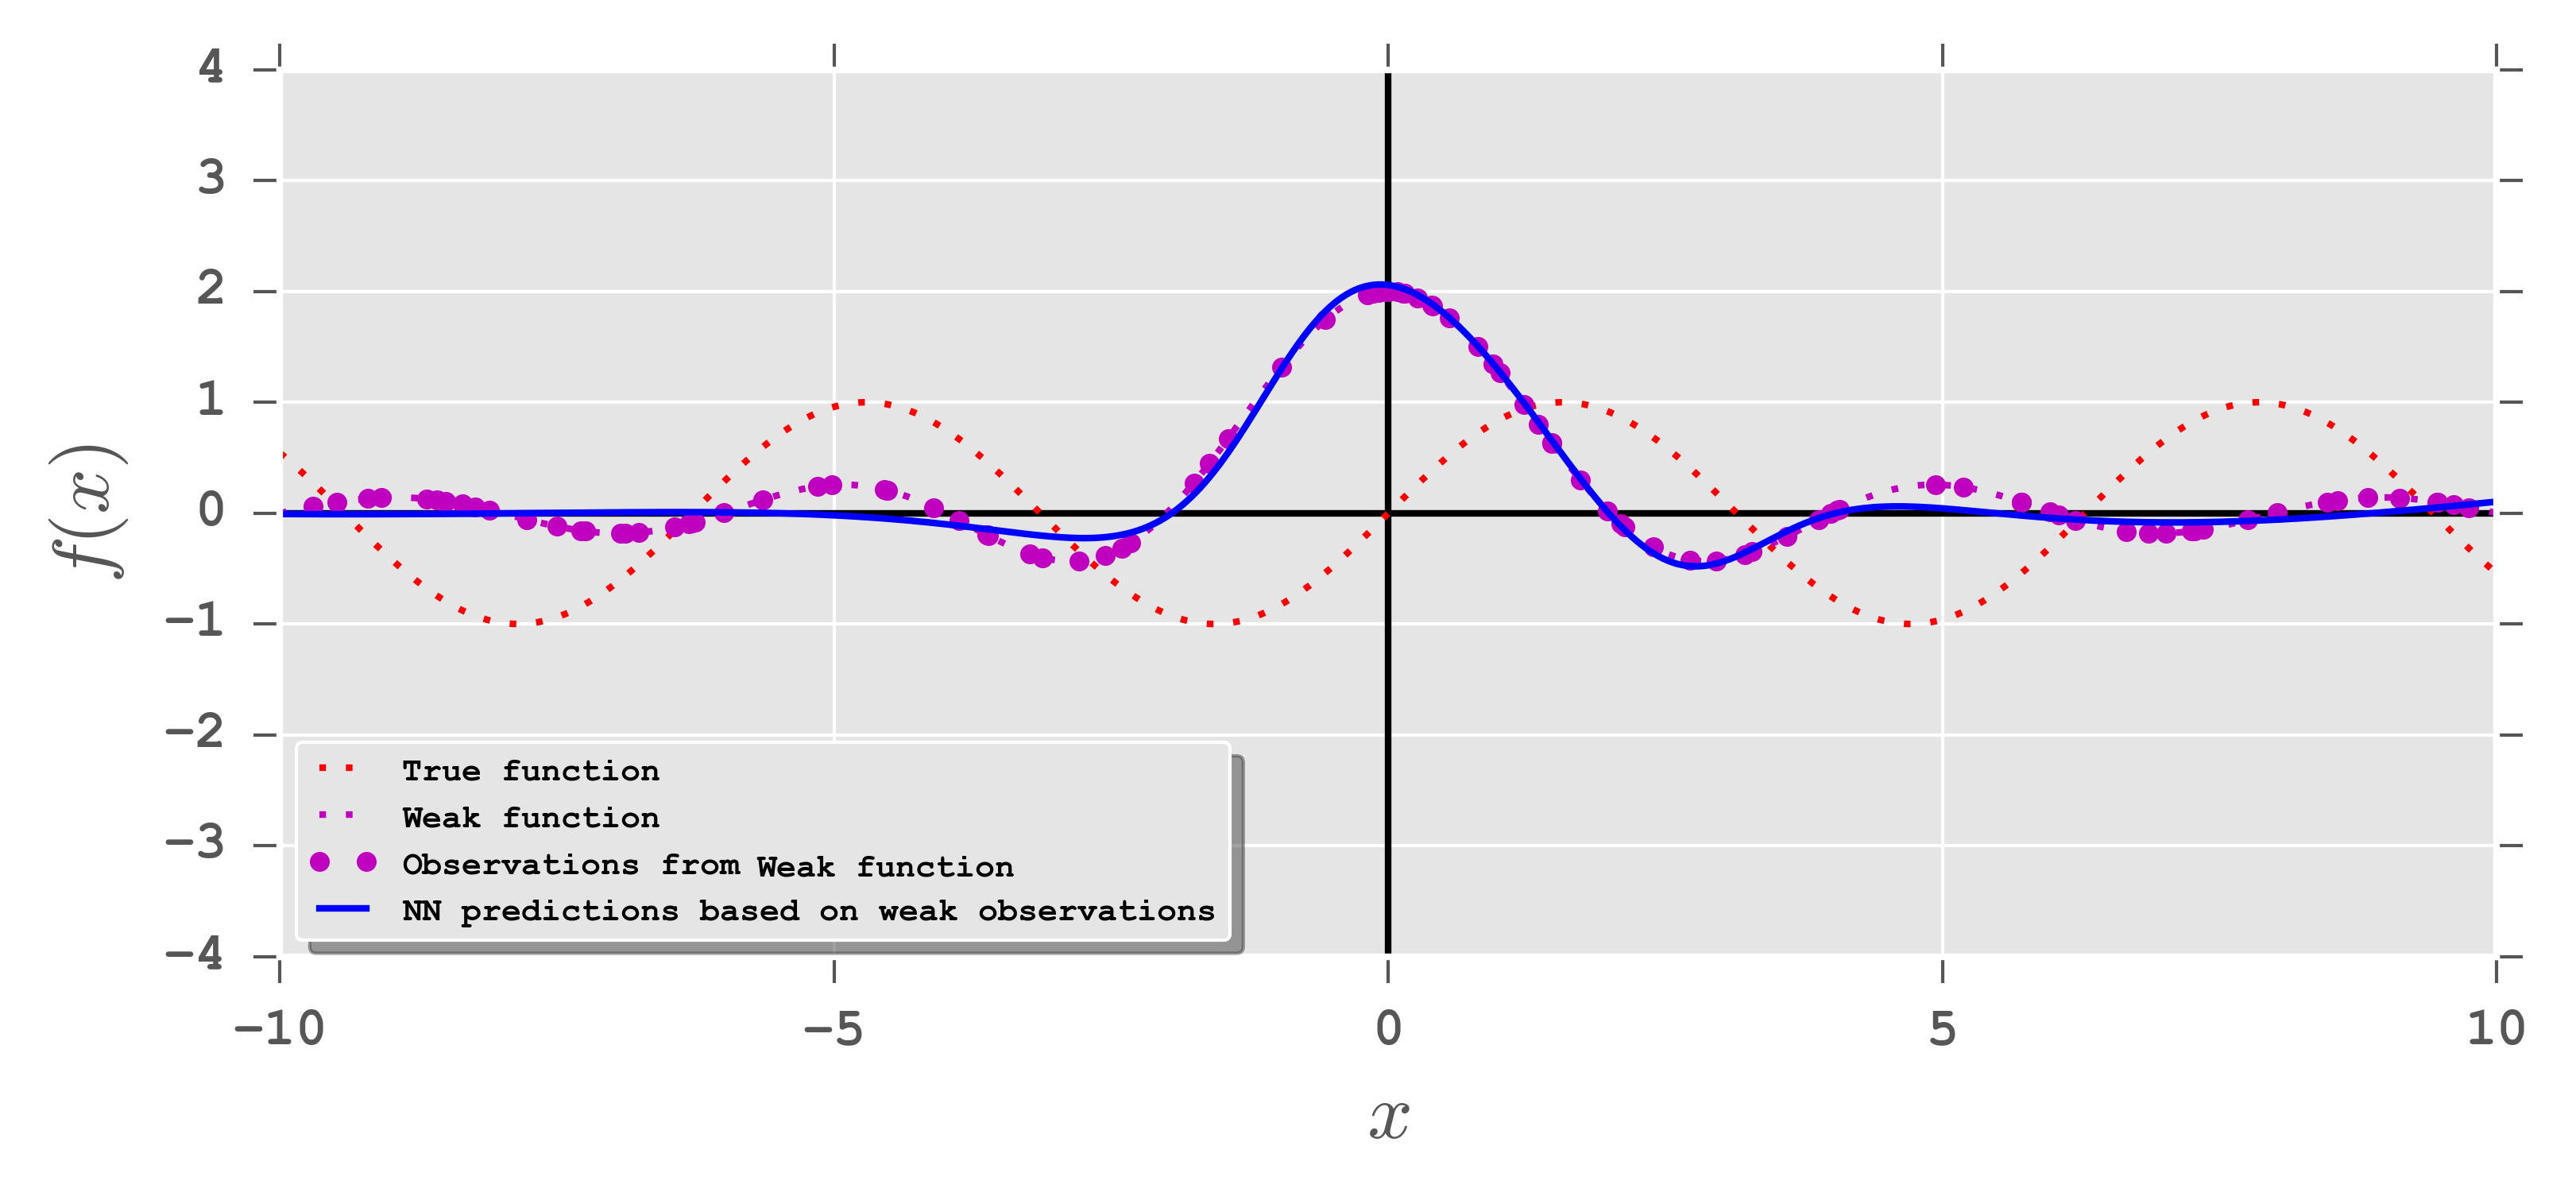
\includegraphics[width=1\textwidth]{03-part-02/chapter-05/figs_and_tables/fig_toy_ex_plot1.png}
        \caption{\label{fig:toy_plot1}Training \std on 100 samples from the weak function.}
    \end{subfigure}%
    ~
    \begin{subfigure}[t]{0.5\textwidth}
        \centering
        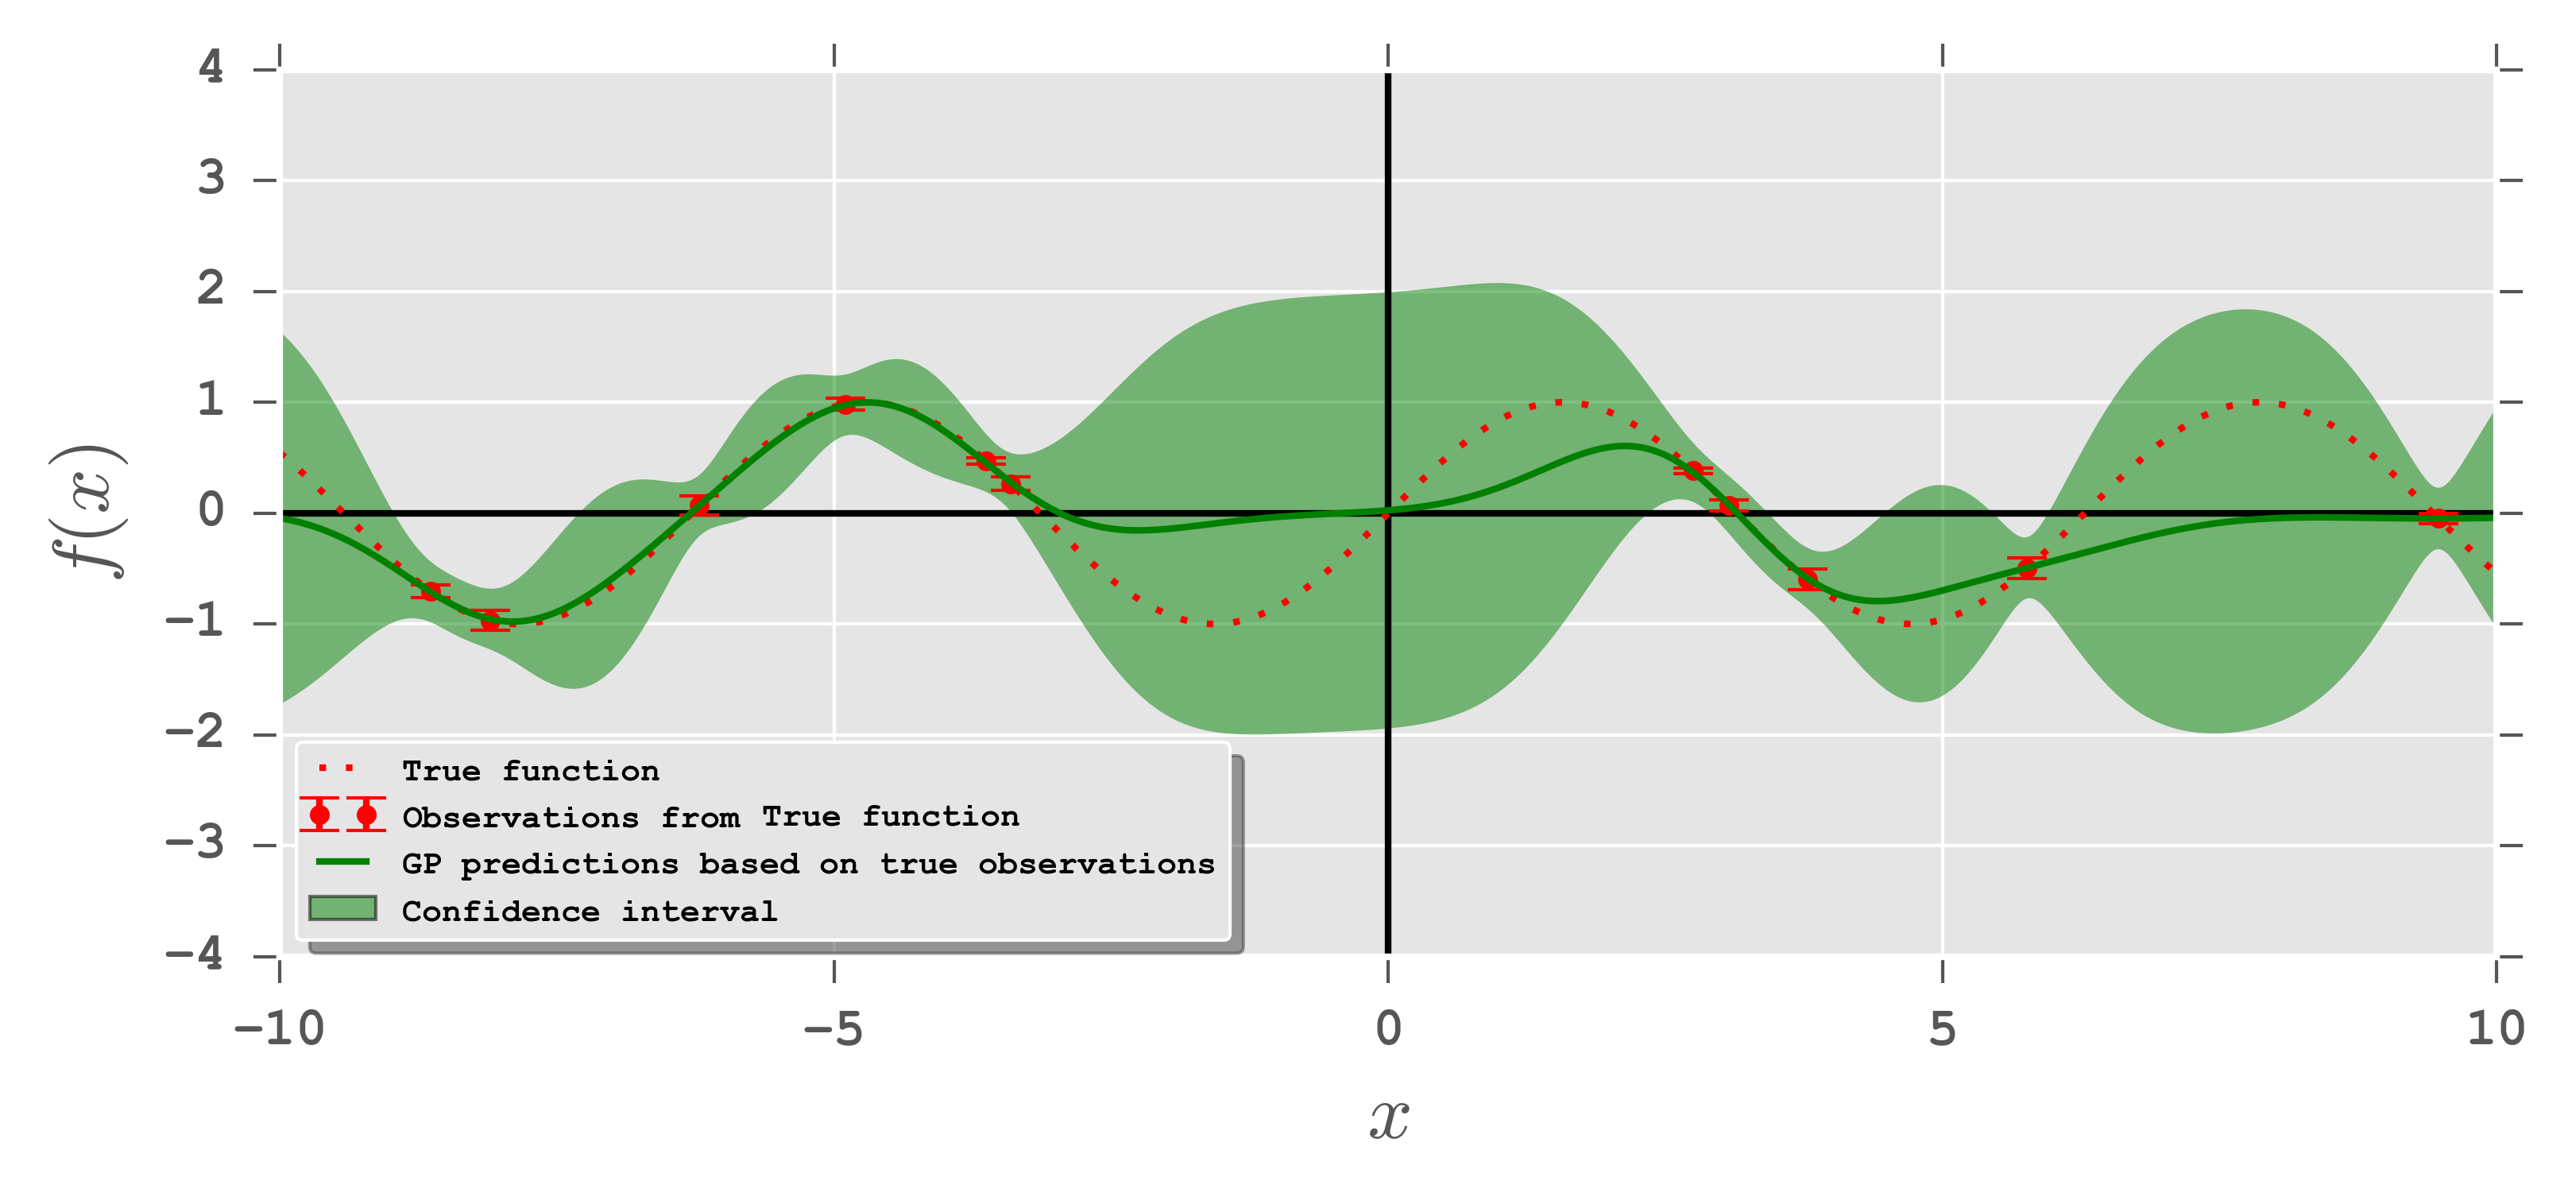
\includegraphics[width=1\textwidth]{03-part-02/chapter-05/figs_and_tables/fig_toy_ex_plot2.png}
        \caption{\label{fig:toy_plot2}Fitting \tch based on 10 observations from the true function.}
    \end{subfigure}%
    }
    \\
    \makebox[\linewidth][c]{%
    \begin{subfigure}[t]{0.5\textwidth}
        \centering
        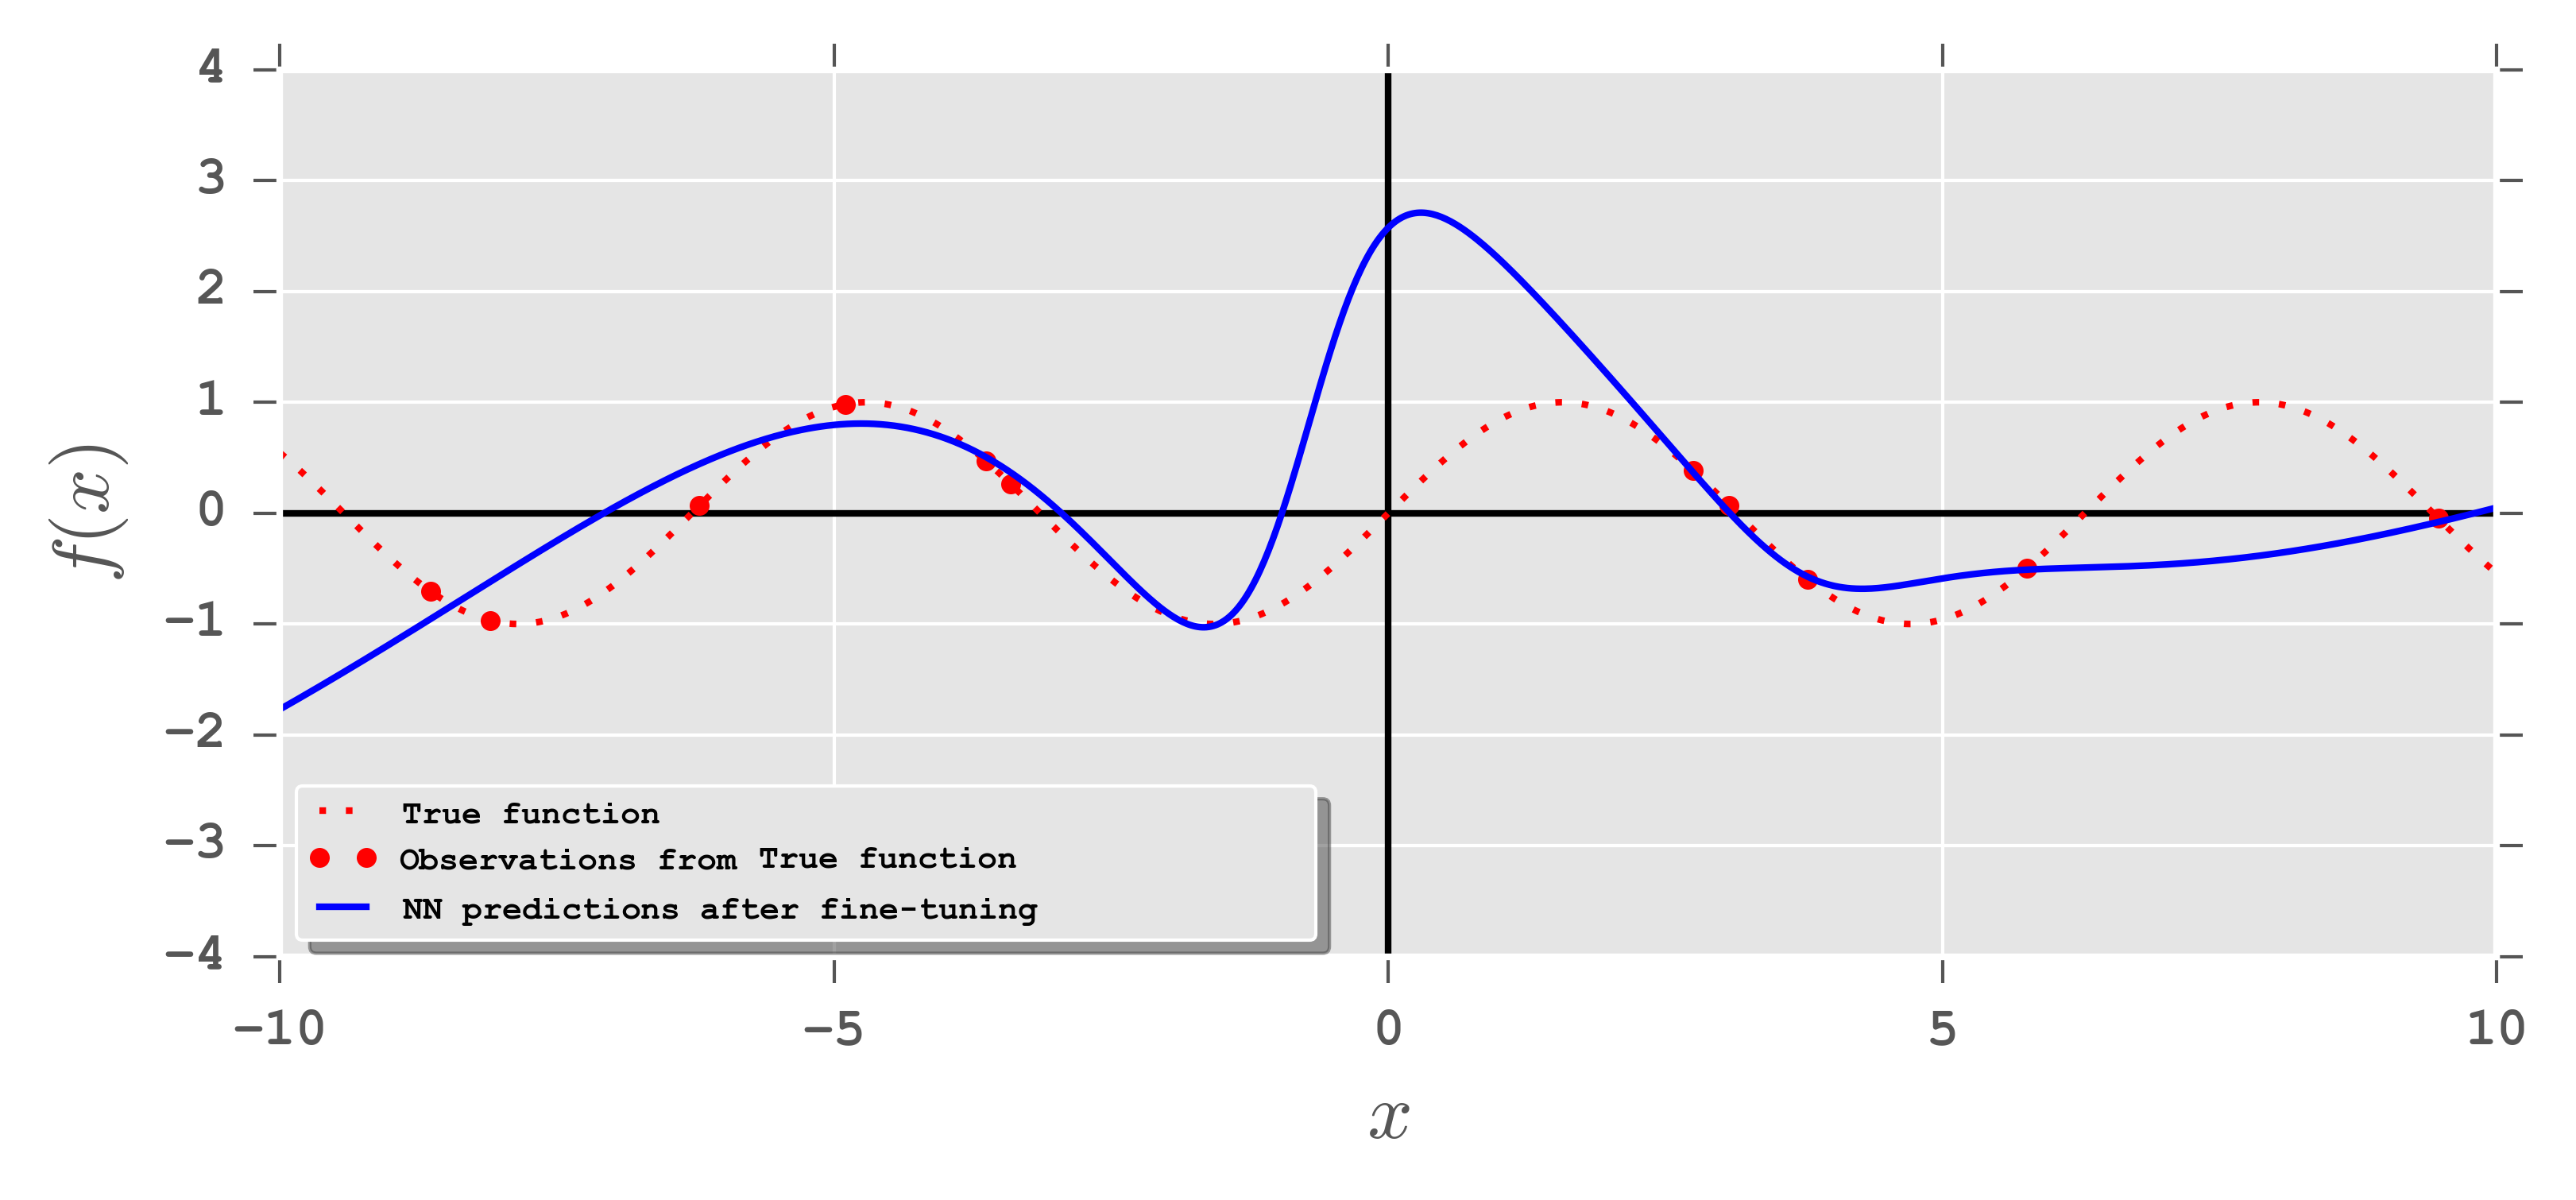
\includegraphics[width=1\textwidth]{03-part-02/chapter-05/figs_and_tables/fig_toy_ex_plot3.png}
        \caption{\label{fig:toy_plot3}Fine-tuning the \std based on observations from the true function.}
    \end{subfigure}%
    ~
    \begin{subfigure}[t]{0.5\textwidth}
        \centering
        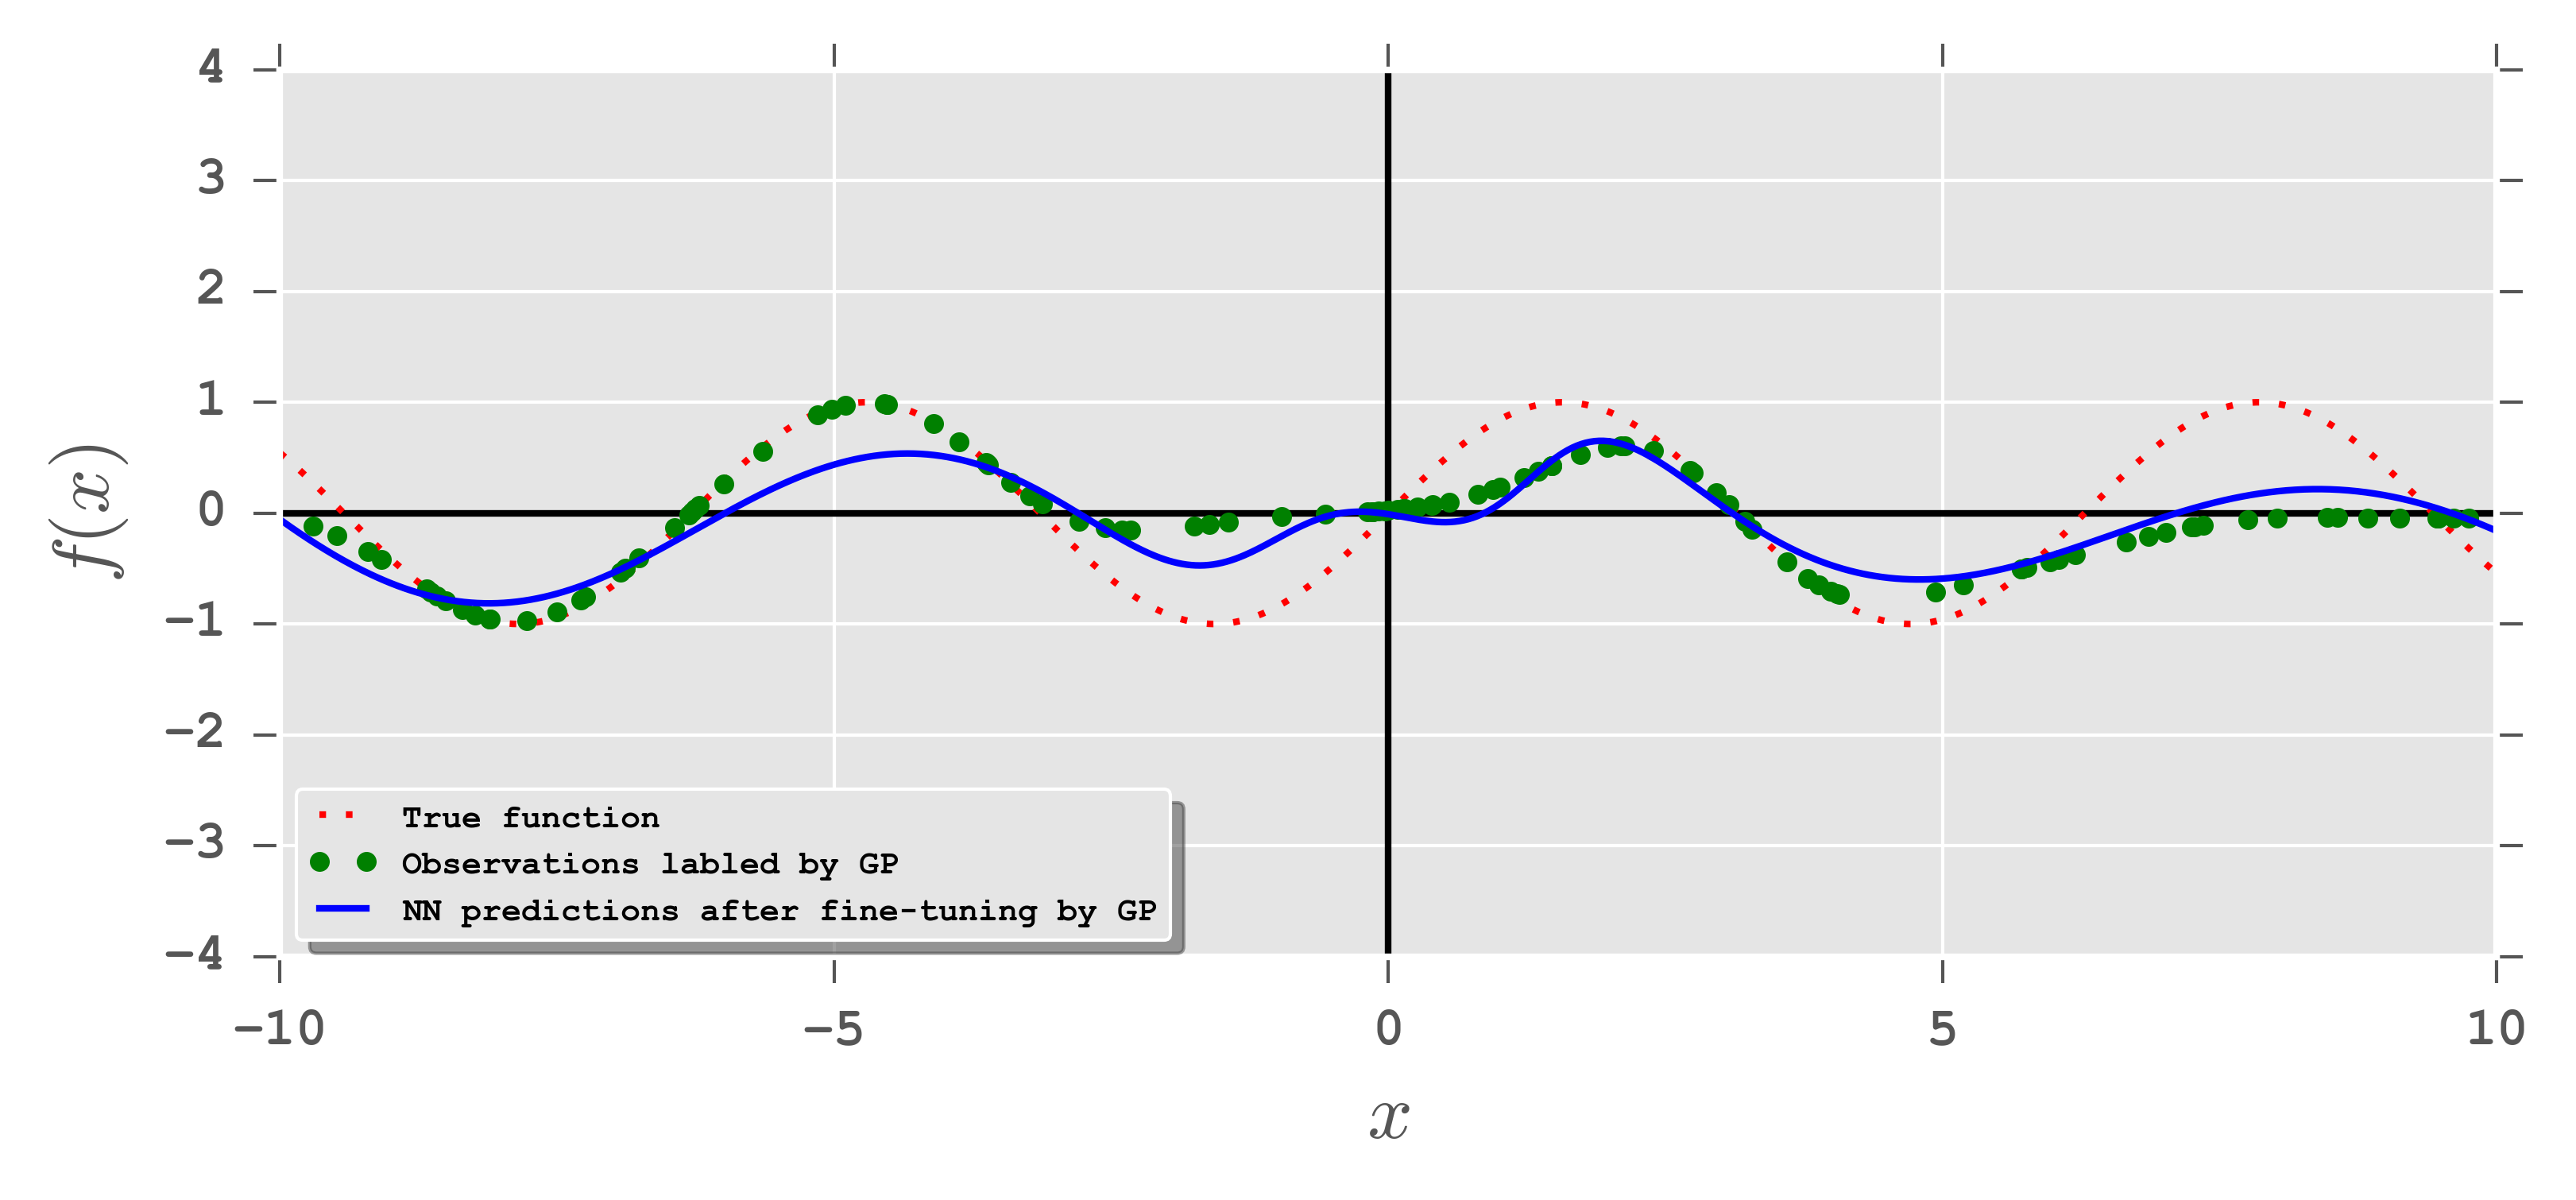
\includegraphics[width=1\textwidth]{03-part-02/chapter-05/figs_and_tables/fig_toy_ex_plot4.png}
        \caption{\label{fig:toy_plot4}Fine-tuning the \std based on label/confidence from \tch.}
    \end{subfigure}%
    }
    \vspace{-5pt}
    \caption{Toy example: The true function we want to learn is $y = \sin(x)$ and the weak function is $y = 2 sinc(x)$.}
    \label{fig:toy}
    \vspace{-5pt}
\end{figure}
To better understand \fwl, we apply \fwl to a one-dimensional toy problem to illustrate the various steps.
%
Let $f_t(x)=\sin(x)$ be the true function (red dotted line in Figure~\ref{fig:toy_plot1}) from which a small set of observations $\mathcal{D}_s=\{x_j,y_j\}$ is provided (red points in Figure~\ref{fig:toy_plot2}). These observation might be noisy, in the same way that labels obtained from a human labeler could be noisy.
%
A \wa function $f_{w}(x)=2sinc(x)$ (magenta line in Figure~\ref{fig:toy_plot1}) is provided, as an approximation to $f_t(.)$.

%
The task is to obtain a good estimate of $f_t(.)$ given the set $\mathcal{D}_s$ of strong observations and the \wa function $f_{w}(.)$.
%
We can easily obtain a large set of observations $\mathcal{D}_w=\{x_i,\tilde{y}_i\}$ from $f_{w}(.)$ with almost no cost (magenta points in Figure~\ref{fig:toy_plot1}). 

As the \tch, we use standard Gaussian process regression\footnote{\url{http://gpflow.readthedocs.io/en/latest/notebooks/regression.html}} with this kernel:
\begin{equation}
k(x_i,x_j)=k_{\rm RBF}(x_i,x_j)+k_{\rm White}(x_i,x_j)
\end{equation}
where,
\begin{flalign*}
    \hspace{6em}
    &&k_{\rm RBF}(x_i,x_j) &= \exp{\left(\frac{\Vert x_i-x_j\Vert^2}{2^2}\right)} & 
    \\
    &&k_{\rm White}(x_i,x_j) &= constant\_value, \quad \forall x_1=x_2 \text{ and } 0 \text{ otherwise} & 
\end{flalign*}

We fit only one $\mathcal{GP}$ on all the data points (i.e., no clustering). Also during fine-tuning, we set $\beta = 1$.
The \std is a simple feed-forward network with the depth of 3 layers and width of 128 neurons per layer.  We have used $tanh$ as the nonlinearity for the intermediate layers and a linear output layer. As the optimizer, we used Adam~\citep{Kingma:2014} and the initial learning rate has been set to $0.001$.
We randomly sample 100 data points from the \wa and 10 data points from the true function. We introduce a small amount of noise to the observation of the true function to model the noise in the human labeled data. 


We consider two experiments: 
\begin{enumerate}[leftmargin=*]
%save some space
\setlength{\topsep}{0.3pt}
\setlength{\partopsep}{0.3pt}
\setlength{\itemsep}{0.3pt}
\setlength{\parskip}{0.3pt}
\setlength{\parsep}{0.3pt}
    \item A neural network trained on weak data and then fine-tuned on strong data from the true function, which is the most common semi-supervised approach (Figure~\ref{fig:toy_plot3}).
    \item A teacher-student framework working by the proposed \fwl approach.
\end{enumerate} 

As can be seen in Figure~\ref{fig:toy_plot4}, \fwl by taking into account label confidence, gives a better approximation of the true hidden function.  We repeated the above experiment 10 times. The average RMSE with respect to the true function on a set of test points over those 10 experiments for the \std, were as follows:
\begin{enumerate}[leftmargin=*]
%save some space
\setlength{\topsep}{0.3pt}
\setlength{\partopsep}{0.3pt}
\setlength{\itemsep}{0.3pt}
\setlength{\parskip}{0.3pt}
\setlength{\parsep}{0.3pt}
    \item Student is trained on weak data (blue line in Figure~\ref{fig:toy_plot1}): $0.8406$,
    \item Student is trained on weak data then fine tuned on true observations (blue line in Figure~\ref{fig:toy_plot3}): $0.5451$,
    \item Student is trained on weak data, then fine tuned by soft labels and confidence information provided by the teacher (blue line in Figure~\ref{fig:toy_plot4}): $0.4143$ (best).
\end{enumerate}